% CVPR 2026 Paper Template
\documentclass[10pt,twocolumn,letterpaper]{article}

% Use final (camera-ready) version
\usepackage{cvpr}

%% This file contains a number of tweaks that are typically applied to the main document.
%% They are not enabled by default, but can be enabled by uncommenting the relevant lines.

%%
%% Inline annotations; for predefined colors, refer to "dvipsnames" in the xcolor package:
%% https://tinyurl.com/overleaf-colors
%%
\newcommand{\red}[1]{{\color{red}#1}}
\newcommand{\todo}[1]{{\color{red}#1}}
\newcommand{\TODO}[1]{\textbf{\color{red}[TODO: #1]}}
%%
%% disable for camera ready / submission by uncommenting these lines  
%%
% \renewcommand{\TODO}[1]{}
% \renewcommand{\todo}[1]{#1}

%%
%% work harder in optimizing text layout. Typically shrinks text by 1/6 of page, enable
%% it at the very end of the writing process, when you are just above the page limit
%%
% \usepackage{microtype}

%%
%% fine-tune paragraph spacing
%%
% \renewcommand{\paragraph}[1]{\vspace{.5em}\noindent\textbf{#1.}}

%%
%% globally adjusts space between figure and caption
%%
% \setlength{\abovecaptionskip}{.5em}


%%
%% Allows "the use of \paper to refer to the project name"
%% with automatic management of space at the end of the word
%%
% \usepackage{xspace}
% \newcommand{\paper}{ProjectName\xspace}

%%
%% Commonly used math definitions
%%
% \DeclareMathOperator*{\argmin}{arg\,min}
% \DeclareMathOperator*{\argmax}{arg\,max}

%%
%% Tigthen underline
%%
% \usepackage{soul}
% \setuldepth{foobar}

\definecolor{cvprblue}{rgb}{0.21,0.49,0.74}
\usepackage[pagebackref,breaklinks,colorlinks,allcolors=cvprblue]{hyperref}

\def\paperID{*****}
\def\confName{CVPR}
\def\confYear{2026}

% ── Additional packages ────────────────────────────────────────────────────────
\usepackage{amsmath,amssymb}
\usepackage{booktabs}
\usepackage{multirow}
\usepackage{enumitem}
\usepackage{subcaption}
\usepackage{tikz}
\usetikzlibrary{arrows.meta,positioning,fit,backgrounds,calc}
\usepackage{parskip}

% ── Macros ─────────────────────────────────────────────────────────────────────
\newcommand{\cifar}{CIFAR-10}
\newcommand{\pp}{\,pp}
\newcommand{\methodA}{Frozen Patch-Whitening}
\newcommand{\methodB}{Dirac Initialisation}
\newcommand{\methodC}{ScaleBias + Lookahead}
\newcommand{\methodD}{Alternating Flip}

\newcommand{\R}{\mathbb{R}}
\newcommand{\transpose}{\mathsf{T}}

% ── Title / Authors ────────────────────────────────────────────────────────────
\title{Do CNN Speed-Up Tricks Transfer to Transformers?\\
    \large Evaluating Fast-Training Techniques on Vision Transformers for \cifar{}}

\author{Siwei LIU\thanks{Equal contribution.}\\
{\tt\small sliudu@connect.ust.hk}
\and
Xingjian ZHANG$^*$\\
{\tt\small xzhangx@connect.ust.hk}
\and
Liwei LI$^*$\\
{\tt\small llix@connect.ust.hk}
\\[4pt]
\normalsize COMP-4471: Deep Learning in Computer Vision --- Course Project\\
\normalsize The Hong Kong University of Science and Technology}

\begin{document}
\maketitle

\begin{abstract}
    Recent work by Garg~\etal~\cite{garg2024cifar10} demonstrated that a carefully engineered CNN can reach $94\%$ accuracy on \cifar{} in 3.29 seconds on a single GPU, using four training tricks: frozen patch-whitening initialisation, Dirac (identity) initialisation, a ScaleBias output layer with the Lookahead optimiser, and alternating horizontal flip.
    We ask whether these tricks transfer to transformer architectures.
    We train a small Vision Transformer (ViT, $\sim$4M parameters) on \cifar{} under two regimes: a weak recipe (100 epochs, basic augmentation, $61.7\%$ baseline) and a strong recipe (300 epochs, RandAugment, Mixup/CutMix, DropPath, $81.4\%$ baseline).
    Under the weak recipe, representation-quality tricks transfer positively (whitening $+1.3$\pp{}, alternating flip $+0.8$\pp{}) while architecture-specific tricks are harmful (Dirac $-7.9$\pp{}, ScaleBias+Lookahead $-16.0$\pp{}).
    Under the strong recipe the picture partially reverses: whitening flips to $-4.4$\pp{} and soft Dirac init ($\alpha{=}0.3$) becomes the only net-positive trick ($+0.4$\pp{}).
    We attribute the whitening reversal to a frozen-embedding/augmentation conflict: filters computed from clean images are mismatched to the heavily transformed inputs of Mixup and CutMix.
    A controlled CNN masked-reconstruction experiment confirms that freezing itself is harmless---only the statistics mismatch matters.
    These findings reveal that the transferability of CNN training tricks depends on the \emph{trick~$\times$~recipe} interaction, not just on architectural compatibility.
\end{abstract}

\section{Introduction}\label{sec:intro}

Training efficiency is a central concern in deep learning for computer vision.
As models grow larger and datasets more complex, reducing the wall-clock time to reach a target accuracy directly lowers research iteration cost and energy consumption.
This problem spans two important settings: \emph{classification}, which assigns an image to a learned class, and \emph{reconstruction}, which predicts masked or corrupted regions of an image.
Both settings have seen rapid architectural progress, from convolutional neural networks (CNNs) to Vision Transformers (ViTs)~\cite{dosovitskiy2021vit}, yet efficient training recipes for these newer architectures remain underdeveloped.

A key gap exists in the transfer of training acceleration techniques.
Garg~\etal~\cite{garg2024cifar10} proposed four methods that dramatically accelerate CNN training on \cifar{}---frozen patch-whitening initialisation, Dirac (identity) initialisation, a ScaleBias output layer with the Lookahead optimiser, and alternating horizontal flip---achieving $94\%$ accuracy in 3.29 seconds on a single {GPU}.
However, it is unknown whether these methods carry their benefits to \emph{transformer} architectures or to \emph{reconstruction} tasks, where the inductive biases and training dynamics differ substantially from CNN classification.
Closing this gap is practically important: practitioners routinely apply CNN-era training recipes to ViTs without systematic validation, potentially wasting or even harming training efficiency.

We address this gap through a controlled empirical study.
We ask: \emph{Do the four CNN speed-up tricks of Garg~\etal{} transfer to (a) ViT-based classification and (b) CNN-based masked reconstruction?}
Our main contributions are:
\begin{enumerate}[leftmargin=*,topsep=2pt,itemsep=1pt]
    \item Two ViT classification baselines on \cifar{}: a \textbf{weak recipe} ($61.7\%$, 100 epochs) and a \textbf{strong recipe} ($81.4\%$, 300 epochs, RandAugment + Mixup/CutMix + DropPath), establishing the accuracy floor against which each trick is measured.
    \item Per-trick ablations under both recipes, isolating the effect of each technique on training efficiency and final accuracy.
    \item An analysis of why the same trick can help under one recipe and hurt under another, identifying the \emph{frozen-whitening/augmentation conflict} as the key mechanism.
    \item A controlled CNN masked-reconstruction experiment that directly tests trick transferability to reconstruction tasks, confirming the conflict mechanism and showing that whitening's benefit is preserved when inputs are unaugmented.
\end{enumerate}

Our central finding is that trick transferability is a \emph{trick~$\times$~recipe} interaction, not a fixed property of the trick or the architecture.
Frozen patch whitening accelerates convergence under basic augmentation ($+1.3$\pp{}) but hurts under strong augmentation ($-4.4$\pp{}); soft Dirac init is the only trick net-positive at the strong recipe level ($+0.4$\pp{}).
Practitioners should evaluate each CNN trick under the full target training recipe and task before adopting it.

The paper is organised as follows. Section~\ref{sec:related} covers related work. Section~\ref{sec:data} describes the dataset and preprocessing. Section~\ref{sec:methods} details the model architecture and each adapted trick. Section~\ref{sec:experiments} presents results, ablations, and mechanistic analyses. Section~\ref{sec:conclusion} concludes.



\section{Related Work}\label{sec:related}

\paragraph{Training acceleration for deep learning.}
Reducing wall-clock training time without sacrificing accuracy is a longstanding goal.
The DAWNBench competition~\cite{coleman2017dawnbench} formalised this as a benchmark, spurring work on cyclic learning rates~\cite{smith2019superconvergence}, mixed-precision training, and large-batch {SGD}.
Garg~\etal~\cite{garg2024cifar10} pushed CNN classification to $94\%$ on \cifar{} in 3.29 seconds using four complementary tricks (patch whitening, Dirac init, ScaleBias+Lookahead, alternating flip).
Our work investigates whether these same acceleration techniques remain effective when the model architecture (CNN $\to$ ViT) or task (classification $\to$ reconstruction) changes.

\paragraph{Vision Transformers on small datasets.}
The original ViT~\cite{dosovitskiy2021vit} required large-scale pretraining to outperform CNNs on small datasets.
DeiT~\cite{touvron2021deit} showed that careful training recipes---knowledge distillation, strong augmentation---allow ViTs to match ResNets without pretraining.
Subsequent work~\cite{touvron2022deit3,liu2021swin} confirmed that augmentation strategy is the dominant factor for ViT efficiency on small datasets.
Our dual-recipe design (weak vs.\ strong augmentation) is motivated directly by this finding: we test whether CNN tricks that help under simple augmentation remain effective under the state-of-the-art ViT recipe.

\paragraph{Masked reconstruction.}
Masked image modelling---predicting corrupted or missing pixel regions---has emerged as a powerful self-supervised objective~\cite{he2022masked}.
CNN encoder-decoders were among the first architectures applied to this task.
We study whether CNN initialisation tricks (whitening, Dirac init) that accelerate classification training also accelerate the convergence of a CNN reconstruction model, extending the scope of the transferability question beyond classification.

\paragraph{Initialisation for transformers.}
ReZero~\cite{bachlechner2021rezero} and T-Fixup~\cite{huang2020improve} propose identity-like initialisations for residual transformer blocks, showing that near-identity starts can remove the need for LR warmup.
Our Dirac init is a stronger variant applied to the attention projections themselves; we show that full identity collapses head diversity, while soft blending ($\alpha{=}0.3$) can be mildly beneficial.

\paragraph{Patch whitening.}
Coates~\etal~\cite{coates2011importance} demonstrated that whitened patch features improve shallow CNN representations.
The original ViT uses a learned linear projection; our work is the first to study frozen whitened patch embeddings under strong augmentation, revealing that the frozen-basis/augmentation statistics mismatch---not freezing per se---is the decisive factor.

\paragraph{Lookahead.}
Zhang~\etal~\cite{zhang2019lookahead} introduced Lookahead as a wrapper that stabilises fast-optimizer trajectories via slow-weight interpolation, validated primarily with flat or mildly decaying LR schedules.
We identify the conflict with monotonically decaying schedules (OneCycleLR, cosine decay) as a distinct failure mode independent of architecture.


\section{Data}
\label{sec:data}

\paragraph{Dataset.}
All experiments use \textbf{CIFAR-10}~\cite{krizhevsky2009cifar}, a standard benchmark for image classification consisting of 60{,}000 colour images ($32\times32$ pixels) evenly distributed across 10 classes (airplane, automobile, bird, cat, deer, dog, frog, horse, ship, truck).
The standard split provides 50{,}000 training images and 10{,}000 test images.

\paragraph{Train/validation split.}
We hold out 10\% of the training set (5{,}000 images) as a validation set for checkpoint selection, leaving 45{,}000 images for training.
The split is determined by a fixed random seed and is identical across all experiments so that validation accuracy is directly comparable.

\paragraph{Preprocessing.}
Raw pixel values in $\{0,\ldots,255\}$ are normalised to $[0,1]$ and then standardised channel-wise using the CIFAR-10 training-set statistics ($\mu = (0.4914, 0.4822, 0.4465)$, $\sigma = (0.2470, 0.2435, 0.2616)$).

\paragraph{Augmentation.}
The two training recipes differ in the augmentation applied during training (validation and test images are always clean):

\begin{itemize}[leftmargin=*,topsep=2pt,itemsep=1pt]
    \item \textbf{Weak recipe:} random $32\times32$ crop from a 4-pixel reflect-padded image, random horizontal flip.
    \item \textbf{Strong recipe:} same crop and flip, followed by RandAugment ($n{=}2$, $m{=}9$), then Mixup ($\alpha{=}0.8$) or CutMix ($\alpha{=}1.0$) applied at the batch level (each with 50\% probability per batch).
\end{itemize}

The key difference between recipes is that Mixup and CutMix blend pairs of images at the pixel level, fundamentally changing the distribution seen by the patch embedding.
This is the mechanism behind the whitening reversal documented in Section~\ref{sec:experiments}: the whitened basis is computed from clean images and therefore mismatches the blended inputs.

\paragraph{Whitening basis.}
For experiments with frozen patch-whitening initialisation, the patch covariance matrix is computed from the first 5{,}000 training images (clean, before any augmentation), using all overlapping $4\times4$ patches.
This is identical to the procedure in the original CNN paper~\cite{garg2024cifar10}.

\section{Methods}\label{sec:methods}

\subsection{Model Architecture}

The input image is split into non-overlapping $4\times4$ patches via a strided Conv2d (the \emph{patch embedding}), producing 64 tokens of dimension 192.
A learnable \texttt{[CLS]} token is prepended, positional embeddings are added, and the resulting 65-token sequence passes through 9 Pre-LN transformer encoder blocks~\cite{dosovitskiy2021vit}.
Each block applies multi-head self-attention (4 heads, dimension 192) followed by a two-layer MLP (hidden dimension 768), both with residual connections.
The \texttt{[CLS]} output at the final block feeds a linear classification head producing 10 logits.
Total trainable parameters: 4{,}028{,}170.

Under the strong recipe, \textbf{stochastic depth} (DropPath~\cite{huang2016deep}) is applied to both residual paths in each block, with rate linearly scaled from 0 to 0.1 across the 9 blocks.
This encourages each block to contribute independently rather than relying on the residual stream, acting as a structured dropout over depth.

\begin{figure}[ht]
    \centering
    \small
    \begin{tabular}{ll}
        \toprule
        Hyperparameter  & Value                   \\
        \midrule
        Image size      & $32\times32$            \\
        Patch size      & $4\times4$ (64 patches) \\
        Embedding dim   & 192                     \\
        Depth           & 9 blocks                \\
        Attention heads & 4 (head dim 48)         \\
        MLP ratio       & 4.0 (hidden 768)        \\
        Dropout         & 0.1                     \\
        Parameters      & 4{,}028{,}170           \\
        \bottomrule
    \end{tabular}
    \captionof{table}{ViT configuration used in all experiments.}\label{tab:vit-config}
\end{figure}

\subsection{Adapting the Four CNN Tricks to ViT}

Each trick was originally designed for the CNN in~\cite{garg2024cifar10}.
We describe each trick, its rationale in the CNN context, and how we adapted it.

\paragraph{Frozen patch-whitening initialisation.}
In the CNN, the first convolutional layer is initialised with whitened PCA filters of the training-set patch covariance, then frozen.
The intent is to provide a rotation-invariant, decorrelated input representation from epoch 0, allowing subsequent layers to focus on learning discriminative features.

We apply the same procedure to the ViT's $4\times4$ Conv2d patch embedding.
Let $\mathbf{\Sigma} = \mathbf{P}^\transpose \mathbf{P}/N$ be the covariance of all $3\times4\times4 = 48$-dimensional patches from the first 5{,}000 training images.
Eigendecomposition gives $\mathbf{\Sigma} = \mathbf{V} \mathbf{\Lambda} \mathbf{V}^\transpose$, and the whitening filters are:
\begin{equation}
    \mathbf{w}_k = -\mathbf{w}_{k+D} =
    \frac{\mathbf{v}_k}{\sqrt{\lambda_k + \varepsilon}},
    \quad k=1,\dots,D,
\end{equation}
filling the first 96 of 192 embedding channels with positive/negative pairs.
The remaining 96 channels retain He initialisation.
The embedding is then frozen for the full training run.

\paragraph{Dirac/identity initialisation.}
In the CNN, the first $C_\text{in}$ filters of each grouped-convolution block are set to the Dirac delta, initialising them as near-identity maps.
This is designed to ensure each block starts as a pass-through, with deviation from the identity learned progressively.

We adapt this to the QKV and output projections of every attention block.
Each of the three $D \times D$ sub-matrices of $\mathbf{W}_\text{QKV} \in \R^{3D \times D}$ is set to $\mathbf{I}_D$, and $\mathbf{W}_O \in \R^{D \times D}$ is set to $\mathbf{I}_D$.
We also test a \emph{soft} variant: $\mathbf{W} \leftarrow \alpha \mathbf{I} + \left( 1 - \alpha \right) \mathbf{W}_\text{rand}$ at $\alpha = 0.3$, blending identity and standard random initialisation.

\paragraph{ScaleBias + Lookahead.}
The CNN appends a fixed \texttt{Scale (1/9)} module after global max-pooling over a $3\times3$ spatial map.
The factor $1/9$ normalises the sum of 9 pooled values.
We generalise to a learnable per-feature affine transform $y_i = s_i x_i + b_i$ (ScaleBias) initialised at $s_i{=}1/9$, replacing the linear head.
The ViT has no analogous pooling (the \texttt{[CLS]} output is a single vector), so the $1/9$ factor is architecturally unmotivated.

Lookahead~\cite{zhang2019lookahead} wraps the base optimiser (AdamW) with a slow-weight update:
\begin{equation}
    \phi_{t+k} \gets \phi_t + \alpha \left( \theta_{t+k} - \phi_t \right),\quad
    \theta \gets \phi_{t+k},
\end{equation}
with $k = 6$, $\alpha = 0.5$.
In the strong recipe we use $s_i = 1.0$ and a cosine LR schedule instead of {OneCycleLR}.

\paragraph{Alternating flip.}
Instead of random horizontal flip (independent Bernoulli ($p{=}0.5$) per sample), we deterministically flip every odd-indexed sample, guaranteeing exactly 50\% flipped images in every epoch with zero batch-level flip-count variance.
The motivation is to reduce gradient noise from inconsistent flip counts within a batch.

Figure~\ref{fig:flip-comparison} illustrates the difference.
In random flip (left), the flip decision is re-drawn each epoch, so the same image may be flipped in one epoch and not the next, and the number of flips per batch varies.
In alternating flip (right), each image has a fixed parity: odd-indexed images are always flipped, even-indexed images are never flipped.
Every epoch and every batch sees exactly the same flip assignment, eliminating the stochastic component entirely.

\begin{figure}[h]
    \centering
    \begin{subfigure}[t]{0.48\linewidth}
        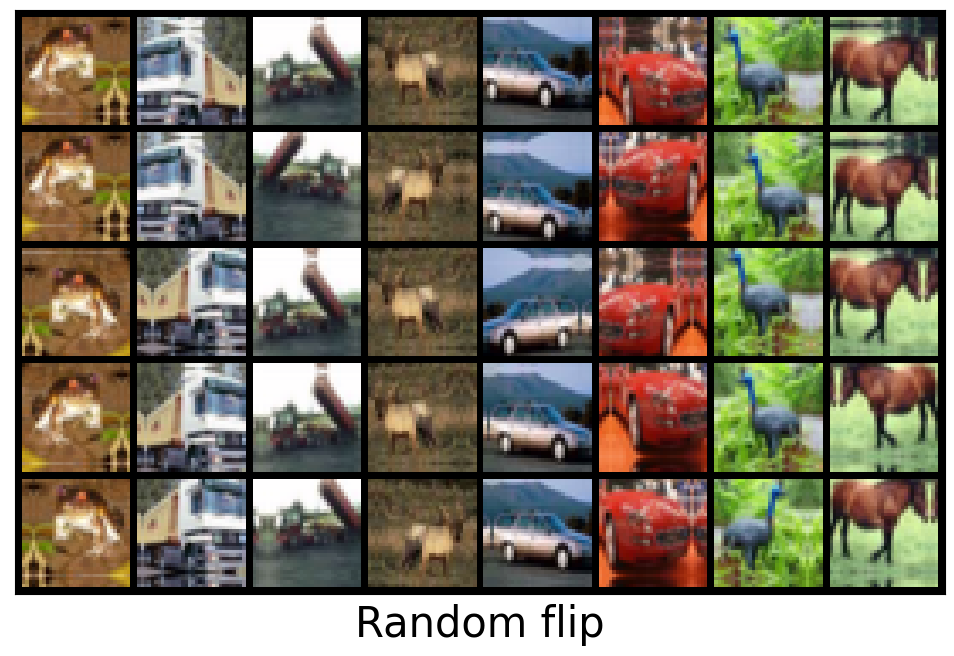
\includegraphics[width=\linewidth]{figures/random_flip.png}
        \caption{Random flip: flip decisions are re-sampled each epoch, producing variable flip patterns across rows.}\label{fig:random-flip}
    \end{subfigure}
    \hfill
    \begin{subfigure}[t]{0.48\linewidth}
        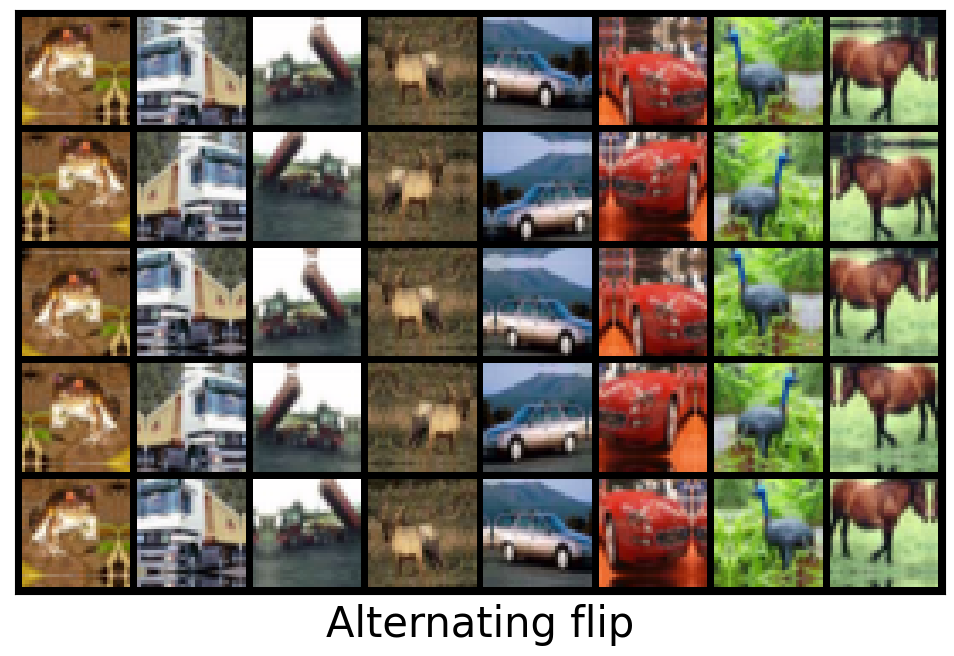
\includegraphics[width=\linewidth]{figures/alternating_flip.png}
        \caption{Alternating flip: each image has a fixed odd/even assignment that repeats identically every epoch.}\label{fig:alt-flip}
    \end{subfigure}
    \caption{Random flip (left) vs.\ alternating flip (right) over five epochs on the same eight \cifar{} images (columns = images, rows = epochs). Random flip produces inconsistent patterns; alternating flip is deterministic and identical across epochs.}\label{fig:flip-comparison}
\end{figure}

\subsection{Training Recipes}

\begin{table}[h]
    \centering
    \setlength{\tabcolsep}{3pt}
    \small
    \begin{tabular}{lll}
        \toprule
        Hyperparameter & Weak             & Strong                          \\
        \midrule
        Epochs         & 100              & 300                             \\
        Peak LR        & $3\times10^{-4}$ & $1\times10^{-3}$                \\
        LR schedule    & OneCycleLR       & Cosine + 5\% warmup             \\
        DropPath       & ---              & 0.1 (linear)                    \\
        Augmentation   & Crop + flip      & Crop + flip + RandAugment       \\
        Mixup / CutMix & ---              & $\alpha{=}0.8$ / $\alpha{=}1.0$ \\
        \bottomrule
    \end{tabular}
    \caption{Training recipe comparison. Both use AdamW, batch size 256, weight decay 0.05, label smoothing 0.1, AMP float16.}\label{tab:recipes}
\end{table}

The weak recipe provides a controlled, low-variance environment for isolating each trick's effect, comparable to the CNN's own training regime.
The strong recipe pushes accuracy to the level achievable with current best-practice ViT training, testing whether the tricks remain useful at the higher baseline.


\section{Experiments}

\label{sec:experiments}

\subsection{Setup}

Experiments run on a single NVIDIA RTX 4090 (24\,GB) per run, four runs in parallel across four GPUs.
All results use the checkpoint with the highest validation accuracy, evaluated on the fixed 10{,}000-image test set.
Each trick is tested in isolation; the ``All methods'' condition applies all four simultaneously.

\subsection{Main Results}

\begin{table*}[ht]
    \centering
    \small
    \begin{tabular}{lrrrr}
        \toprule
        \multirow{2}{*}{Experiment}                            &
        \multicolumn{2}{c}{Weak recipe (100 ep, 61.68\% base)} &
        \multicolumn{2}{c}{Strong recipe (300 ep, 81.42\% base)}
        \\
        \cmidrule(lr){2-3}\cmidrule(lr){4-5}                   &
        Test Acc.                                              &
        $\Delta$                                               &
        Test Acc.                                              &
        $\Delta$
        \\
        \midrule
        Baseline                                               &
        61.68\%                                                &
        ---                                                    &
        81.42\%                                                &
        ---
        \\
        \midrule
        + \methodA{}                                           &
        \textbf{62.99\%}                                       &
        $+1.31$\pp{}                                           &
        77.03\%                                                &
        $-4.39$\pp{}
        \\
        + \methodD{}                                           &
        62.48\%                                                &
        $+0.80$\pp{}                                           &
        80.60\%                                                &
        $-0.82$\pp{}
        \\
        + \methodB{} (full, $\alpha{=}1.0$)                    &
        53.78\%                                                &
        $-7.90$\pp{}                                           &
        79.20\%                                                &
        $-2.22$\pp{}
        \\
        + \methodB{} (soft, $\alpha{=}0.3$)                    &
        60.52\%                                                &
        $-1.16$\pp{}                                           &
        \textbf{81.83\%}                                       &
        $+0.41$\pp{}
        \\
        + \methodC{}                                           &
        45.71\%                                                &
        $-15.97$\pp{}                                          &
        76.39\%                                                &
        $-5.03$\pp{}
        \\
        \midrule
        All methods                                            &
        38.05\%                                                &
        $-23.63$\pp{}                                          &
        71.74\%                                                &
        $-9.68$\pp{}
        \\
        \bottomrule
    \end{tabular}
    \caption{Test accuracy under both training recipes. $\Delta$ is relative to the corresponding baseline.
    Strong-recipe \methodC{} uses $s_i{=}1.0$ and cosine LR.
    Bold marks the best single-trick result per recipe.}
    \label{tab:results}
\end{table*}

Table~\ref{tab:results} shows the main results.
Under the \textbf{weak recipe}, whitening ($+1.31$\pp{}) and alternating flip ($+0.80$\pp{}) are net-positive; Dirac and ScaleBias+Lookahead are harmful ($-7.90$\pp{} and $-15.97$\pp{}); all methods combined yields the worst result ($-23.63$\pp{}).
Under the \textbf{strong recipe}, the ordering shifts: whitening flips to $-4.39$\pp{}, Dirac (full) narrows to $-2.22$\pp{}, and soft Dirac ($\alpha{=}0.3$) becomes the only net-positive trick ($+0.41$\pp{}).

\begin{table}[ht]
    \centering
    \setlength{\tabcolsep}{3pt}
    \small
    \begin{tabular}{rcccccc}
        \toprule
        Ep  & Base          & Alt           & White         & Dirac & SB+LA & All  \\
        \midrule
        50  & 47.8          & 49.7          & \textbf{53.4} & 41.2  & 40.2  & 44.8 \\
        100 & 61.6          & 60.9          & \textbf{60.5} & 53.4  & 53.3  & 55.7 \\
        150 & 68.2          & \textbf{69.3} & 65.2          & 63.6  & 63.2  & 61.2 \\
        200 & 71.9          & \textbf{73.8} & 68.8          & 69.6  & 67.8  & 65.3 \\
        250 & 75.7          & \textbf{77.3} & 73.8          & 74.7  & 71.5  & 68.3 \\
        300 & \textbf{81.1} & 81.0          & 77.0          & 79.2  & 75.3  & 70.8 \\
        \bottomrule
    \end{tabular}
    \caption{Validation accuracy (\%) at selected epochs, strong recipe.}
    \label{tab:epochs}
\end{table}

Table~\ref{tab:epochs} traces convergence under the strong recipe.
Whitening leads at epoch 50 (53.4\%) but is overtaken by epoch 150 as the frozen basis becomes mismatched to the increasingly augmented input distribution.

\begin{figure*}[ht]
    \centering
    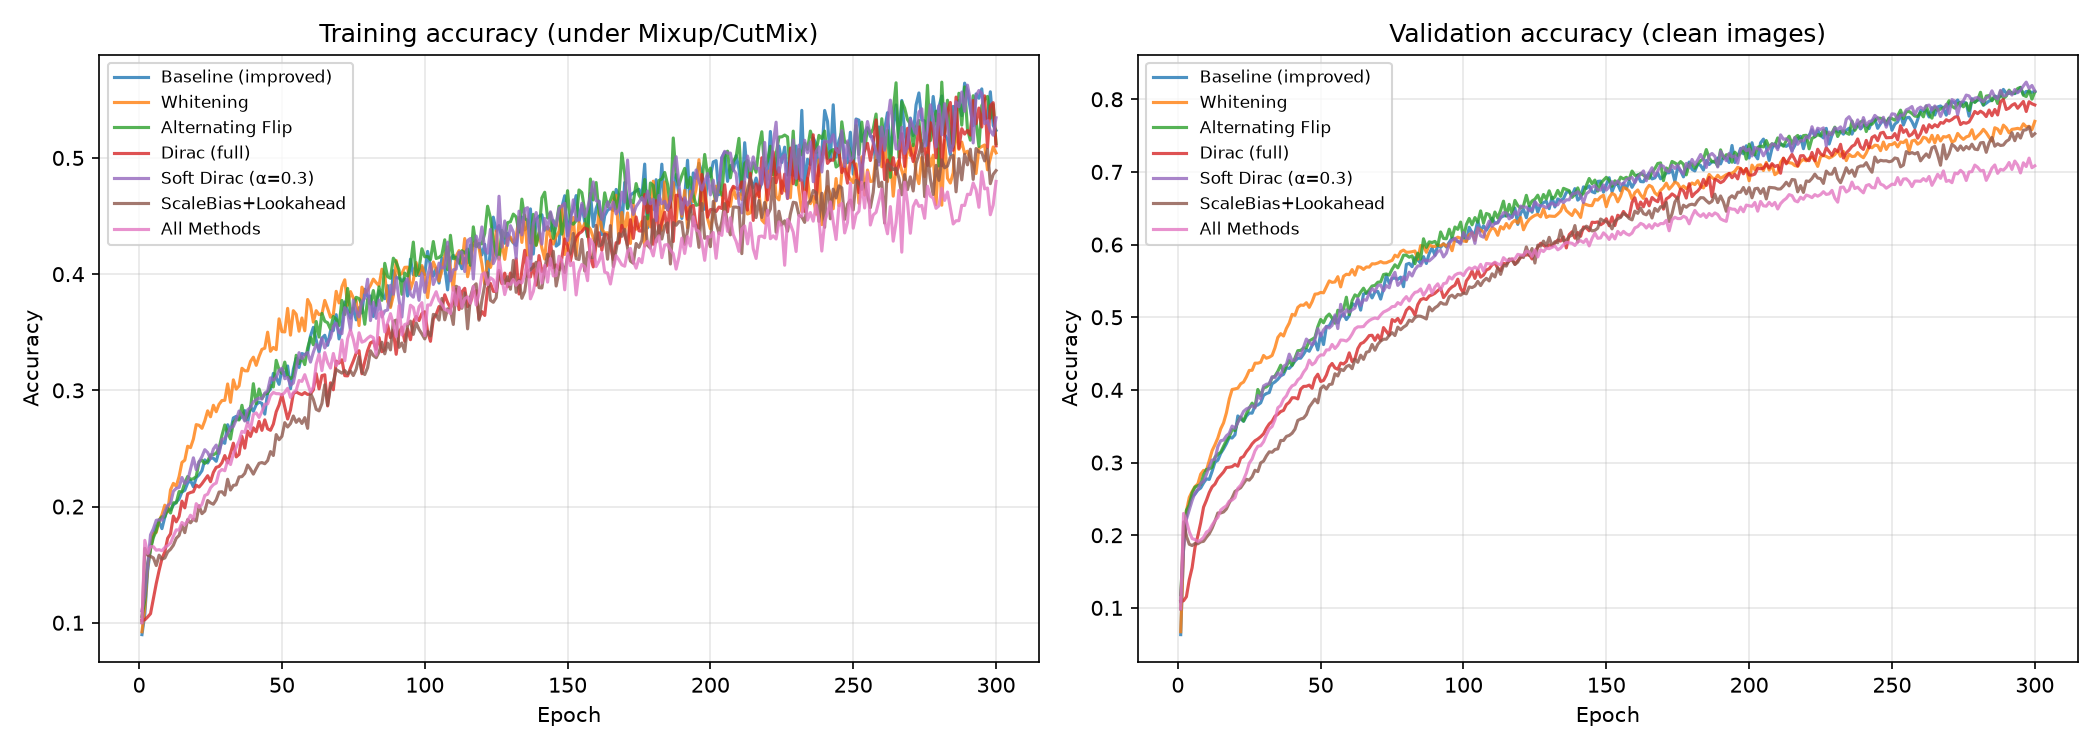
\includegraphics[width=\linewidth]{figures/comparison_v3.png}
    \caption{Validation accuracy over 300 epochs (strong recipe). Soft Dirac and Alternating Flip track the baseline; Whitening, ScaleBias+Lookahead, and All Methods fall behind.}
    \label{fig:curves}
\end{figure*}

\subsection{Why Whitening Reverses Under the Strong Recipe}

The whitened filters are eigenvectors of the patch covariance computed from \emph{clean} training images, then frozen.
Under the strong recipe, Mixup and CutMix blend pairs of images pixel-by-pixel, producing inputs whose patch statistics differ substantially from the clean-image basis.
Because the embedding is frozen, it cannot adapt.

\paragraph{CNN reconstruction confirms the mechanism.}
To isolate this effect, we run a controlled masked-pixel reconstruction experiment: a CNN encoder-decoder predicts the RGB values of 32 randomly masked $4\times4$ blocks per image, with \emph{no} augmentation beyond masking.

\begin{figure}[ht]
    \centering
    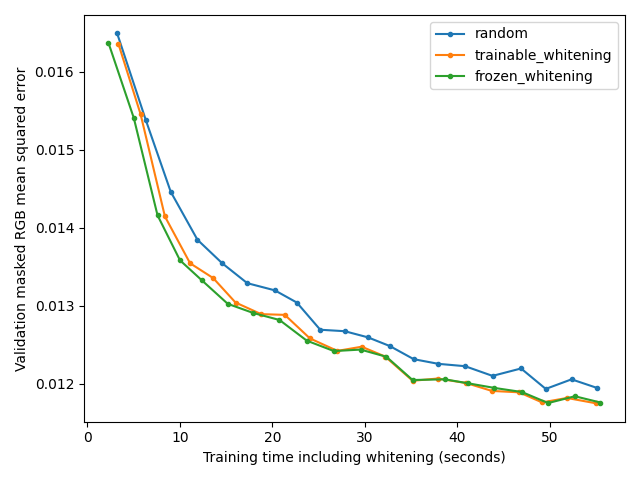
\includegraphics[width=\linewidth]{figures/cnn_reconstruction.png}
    \caption{Masked RGB reconstruction MSE over 20 epochs (lower is better). Both whitening variants beat the random baseline. Trainable and frozen whitening are nearly identical, confirming that freezing itself does not hurt---only the input-distribution mismatch does.}
    \label{fig:reconstruction}
\end{figure}

As Figure~\ref{fig:reconstruction} shows, both trainable and frozen whitening outperform the random baseline at every epoch (final MSE: 0.01175 / 0.01176 vs.\ 0.01195, $\sim$1.7\% relative improvement).
Critically, trainable and frozen whitening differ by only $\Delta = 0.000009$ MSE, confirming that \emph{freezing itself is not harmful}.
The reversal in the classification task therefore stems entirely from the mismatch between the frozen basis and the augmented inputs.

\subsection{All Tricks on CNN Reconstruction}

We extend the reconstruction study to test all four tricks individually and combined, using the same masked-RGB task with 20 epochs and no augmentation beyond masking.
Table~\ref{tab:recon} reports the final validation MSE, and Figure~\ref{fig:reconstruction_full} shows the convergence curves.

\begin{table}[ht]
    \centering
    \small
    \setlength{\tabcolsep}{4pt}
    \begin{tabular}{lrr}
        \toprule
        Variant           & Val MSE (ep 20) & $\Delta$ vs baseline \\
        \midrule
        Baseline          & 0.012207 & ---           \\
        \midrule
        Frozen whitening  & 0.012042 & $-$1.35\%     \\
        Alternating flip  & 0.012116 & $-$0.75\%     \\
        ScaleBias         & 0.012016 & $-$1.56\%     \\
        Dirac init        & 0.011982 & $-$1.84\%     \\
        Lookahead         & \underline{0.011581} & $-$5.12\% \\
        \midrule
        All methods       & \textbf{0.011075} & $-$9.27\% \\
        \bottomrule
    \end{tabular}
    \caption{Final validation MSE on masked RGB reconstruction (lower is better).
        $\Delta$ is relative improvement over the baseline MSE.}
    \label{tab:recon}
\end{table}

\begin{figure}[ht]
    \centering
    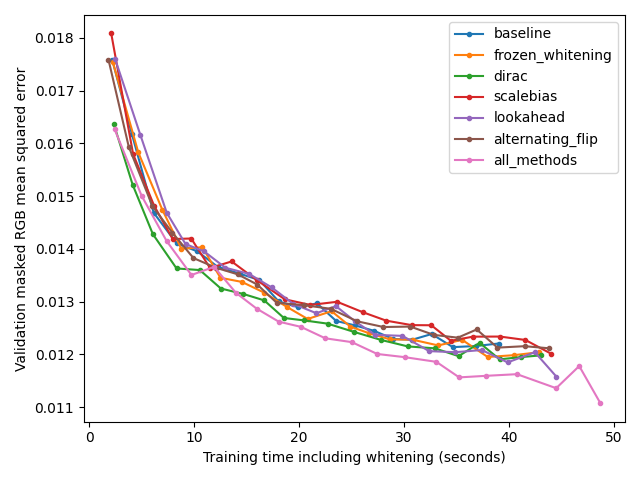
\includegraphics[width=\linewidth]{figures/cnn_reconstruction_full.png}
    \caption{MSE convergence over 20 epochs for all trick variants on CNN masked reconstruction.
        All tricks improve over the baseline; Lookahead is the strongest single trick, and all methods combined achieves the best result.}
    \label{fig:reconstruction_full}
\end{figure}

The results tell a strikingly different story from the ViT classification experiments.
\emph{All} tricks reduce validation MSE, every single trick is helpful, and they compose constructively: all methods combined achieves $-9.27\%$ relative improvement, the best result.

Three observations explain why reconstruction behaves differently from classification.

\textbf{(1) Frozen whitening works because there is no augmentation conflict.}
Masking preserves the patch covariance of the original images, so the frozen whitened basis remains matched to the actual inputs throughout training.
The $-1.35\%$ improvement mirrors the weak-recipe ViT result ($+1.31$\pp{}) and directly confirms that the reversal under the strong recipe was caused by augmentation mismatch, not by freezing.

\textbf{(2) Lookahead is the strongest single trick ($-5.12\%$).}
In the ViT experiments, Lookahead conflicted with the cyclic LR schedule.
Here, we use a flat Adam LR for the reconstruction model---the regime for which Lookahead was originally validated.
Without the schedule conflict, its slow-weight stabilisation reduces oscillation and produces smooth, monotonic convergence.
This directly validates our diagnosis from the ViT experiments: Lookahead's harmful interaction was with the decaying LR schedule, not with learning in general.

\textbf{(3) Dirac init helps in a CNN reconstruction model.}
Unlike in the ViT, where Dirac init collapses self-attention heads into a uniform transformation, the CNN's grouped convolutions are not subject to the same symmetry pathology.
Near-identity initialisation allows early layers to act as pass-throughs while the decoder learns to predict masked regions, and specialisation emerges gradually.
The $-1.84\%$ improvement is consistent with its intended behaviour in the original paper.

Together, these results complete the transferability picture.
When tricks are tested on the architecture and task they were designed for (or on a task that avoids their known failure modes), they are uniformly effective and compose well.
The failures observed in ViT classification are not intrinsic to the tricks themselves but arise from specific mismatches: frozen whitening with strong augmentation, Dirac init with attention symmetry, and Lookahead with decaying LR schedules.

\subsection{Why Dirac Init Improves With Strong Augmentation}

Full identity initialisation collapses all attention heads to the same transformation at epoch 0:
\begin{equation}
    \operatorname{Attn}(X) =
    \operatorname{softmax} \!\left(
    \frac{XX^\transpose}{\sqrt{d}}
    \right) X.
\end{equation}
The model must break this symmetry before specialising, wasting early training.
Under the weak recipe this costs $-7.90$\pp{}; under the strong recipe Mixup/CutMix supply the gradient diversity needed to break symmetry faster, narrowing the gap to $-2.22$\pp{}.
Soft Dirac ($\alpha=0.3$) avoids the full collapse while retaining a mild identity prior, turning net-positive under the strong recipe ($+0.41$\pp{}).

\subsection{Why ScaleBias + Lookahead Hurts}

Two independent issues compound.
First, initialising ScaleBias with $s_i{=}1/9$ suppresses gradients reaching the transformer body by $0.11\times$; fixing to $s_i{=}1.0$ removes this.
Second, Lookahead's slow-weight pull ($\phi\gets\phi+\alpha(\theta-\phi)$, $\theta\gets\phi$) partially reverses fast-weight progress every $k$ steps.
Under a flat LR the fast weights converge in a consistent direction, so the pull is benign.
Under OneCycleLR or cosine decay, the direction changes substantially across $k$ steps, introducing conflicting gradient history.
The residual $-5.03$\pp{} after both fixes suggests that only a flat LR fully decouples Lookahead from the schedule.

\subsection{Discussion}

The results reveal two orthogonal axes of compatibility:
\begin{enumerate}[leftmargin=*,topsep=2pt,itemsep=1pt]
    \item \textbf{Architectural:} Dirac init and post-pooling output scaling assume convolutional structure and remain net-negative in transformers (though gaps narrow with appropriate fixes).
    \item \textbf{Recipe:} Frozen whitening and Lookahead depend on training-recipe properties (augmentation statistics, LR schedule shape) independently of architecture.
\end{enumerate}
The ``All methods combined'' condition is the worst result under both recipes, confirming that the failure modes are additive rather than self-cancelling.

\section{Conclusion}
\label{sec:conclusion}

We evaluated four fast-training techniques from a state-of-the-art CNN recipe on a Vision Transformer trained on \cifar{}, under both a weak recipe ($61.7\%$ baseline) and a strong recipe ($81.4\%$ baseline).

Under the weak recipe, representation-quality tricks transfer positively (whitening $+1.3$\pp{}, alternating flip $+0.8$\pp{}) while architecture-specific tricks are harmful (Dirac $-7.9$\pp{}, ScaleBias+Lookahead $-16.0$\pp{}).
Under the strong recipe the picture partially reverses, with whitening flipping to $-4.4$\pp{} and soft Dirac becoming the only net-positive trick ($+0.4$\pp{}).

The central lesson is that trick transferability is a \emph{trick~$\times$~recipe} interaction, not a fixed architectural property.
Frozen whitening is beneficial only when training augmentation preserves the patch statistics of the whitening basis; Mixup and CutMix destroy that match.
Dirac init is harmful when augmentation is too weak to quickly break attention symmetry, and mildly helpful when it is strong enough.
Lookahead conflicts with any monotonically decaying LR schedule regardless of architecture.

A controlled CNN masked-reconstruction experiment directly confirmed the whitening mechanism: trainable and frozen whitening perform identically when inputs are unaugmented, isolating the input-distribution mismatch as the sole cause of the reversal.

\paragraph{Future work.}
The most direct next steps are: (1) learnable (unfrozen) whitening, which should recover whitening's benefit under strong augmentation; (2) decayed soft Dirac ($\alpha$ annealed to 0), which may turn further positive; (3) Lookahead paired with a flat LR to remove the schedule conflict; and (4) an all-methods combination using all three fixes, to test whether the corrected tricks compose additively.


{
    \small
    \bibliographystyle{ieeenat_fullname}
    \bibliography{references}
}

\end{document}
